%
% Complete documentation on the extended LaTeX markup used for Insight
% documentation is available in ``Documenting Insight'', which is part
% of the standard documentation for Insight.  It may be found online
% at:
%
%     http://www.itk.org/

\documentclass{InsightArticle}


%%%%%%%%%%%%%%%%%%%%%%%%%%%%%%%%%%%%%%%%%%%%%%%%%%%%%%%%%%%%%%%%%%
%
%  hyperref should be the last package to be loaded.
%
%%%%%%%%%%%%%%%%%%%%%%%%%%%%%%%%%%%%%%%%%%%%%%%%%%%%%%%%%%%%%%%%%%
\usepackage[dvips,
bookmarks,
bookmarksopen,
backref,
colorlinks,linkcolor={blue},citecolor={blue},urlcolor={blue},
]{hyperref}
% to be able to use options in graphics
\usepackage{graphicx}
% for pseudo code
\usepackage{listings}
% subfigures
\usepackage{subfigure}


%  This is a template for Papers to the Insight Journal. 
%  It is comparable to a technical report format.

% The title should be descriptive enough for people to be able to find
% the relevant document. 
\title{WrapITK: Enhanced languages support\\ for the Insight Toolkit}

% Increment the release number whenever significant changes are made.
% The author and/or editor can define 'significant' however they like.
\release{0.1}

% At minimum, give your name and an email address.  You can include a
% snail-mail address if you like.
\author{Ga\"etan Lehmann{$^1$}{\small{,}} Zachary Pincus{$^2$} {\small{and}} Benoit Regrain{$^3$}}
\authoraddress{{$^1$}Unit\'e de Biologie du D\'eveloppement et de la Reproduction, Institut National de la Recherche Agronomique, 78350 Jouy-en-Josas, France\\
{$^2$}Program in Biomedical Informatics and Department of Biochemistry, Stanford University School of Medicine, Stanford, California\\
{$^3$}CREATIS, CNRS UMR 5515, 69621 Villeurbanne, France}

\begin{document}
\lstset{language=python}
\maketitle

\ifhtml
\chapter*{Front Matter\label{front}}
\fi


\begin{abstract}
\noindent
ITK \cite{ITKWebSite} is a huge image analysis library, which contains lots of state of the arts
algorithms implementations. However, using it in C++ can be difficult and is
definitively bad suited for prototyping. WrapITK aims to allow classes from ITK
(and custom, classes that interact with ITK) to be "wrapped" for use with
languages like Python \cite{PythonWebSite}, Tcl \cite{TclWebSite}, and Java \cite{JavaWebSite}.
\end{abstract}

\tableofcontents

\section{Introduction}

WrapITK is a project designed to allow classes from ITK (and custom, classes
that interact with ITK) to be "wrapped" for use with languages like
Python \cite{PythonWebSite}, Tcl \cite{TclWebSite}, and Java \cite{JavaWebSite}.

Note that ITK already has a wrapping infrastructure, and that WrapITK is based
on it, and use the same tools: CMake \cite{CMakeWebSite}, GCC-XML \cite{GccxmlWebsite}
and CableSwig\footnote{CableSwig is based on a now quite old version of SWIG
\cite{SwigWebSite}.} \cite{CableSwigWebSite}. This project aims to
address the following deficits of the existing wrappers (and others):
\begin{itemize}
  \item  ITK is a huge library, but only a small number of classes are available
in target languages. It become quickly frustrating for the user, especially when
he has to spend lot of time to extend the current set of classes. Even if it is
not yet complete, the WrapITK's set of classes have been highly extended. Moreover,
the user can choose at build time which types and which dimensions he want to wrap.

  \item  The template arguments set is poorly chosen, making sometime impossible
to create a pipeline. In WrapITK, most of the filters have the same input and output
types, and only a few filters allow to change type. This make the types manipulated 
by filters more consistent, and the user should always be able to build his pipeline.

  \item  Lots of types returned by ITK object's methods are not usable in target
languages. For example, the \verb$GetPixel()$ method of the class \verb$itk::Image$
returns a string describing a pointer, but don't return the pixel value. In WrapITK,
most types used in classes are available in target languages.

  \item  Names in target languages are inconsistent. WrapITK use a strict naming
convention which should make easier to identify the template arguments.

  \item  The ITK wrapping system is difficult to understand and maintain. WrapITK was
written - and thoroughly documented - to be as easy as possible to understand,
maintain, and extend.

  \item  It is non-trivial to add wrappers for different ITK classes to the system. In
WrapITK, adding a wrapper can be as simple as adding a single file containing a
few well-documented cmake macros.

  \item  It is difficult if not impossible to add original-style ITK wrappers for
external C++ classes that interact with ITK. WrapITK provides explicit hooks for
external C++ classes to be wrapped and even installed in the WrapITK tree so
that they interact seamlessly with the other wrapped classes.

  \item  The python's \verb$InsightToolkit$ module is only structured as a big
list of names. It make it nearly unusable in the python interpreter. WrapITK
comes with a new well designed python module easy to use in interpreter, and
providing run-time lookup of templated types - thing which can't be easily done
in C++. Additionally, WrapITK ensures that \verb$SmartPointer$s are always
returned and acceptable as input, so no bare pointers are ever exposed to
Python. This is not the case in the standard ITK wrappers.

  \item ITK was broken on MacOS X \cite{MacOsXWebSite} with python.

\end{itemize}

Currently, WrapITK have been tested on Mandriva Linux \cite{MandrivaWebSite}, and MacOS X, and only
supports Python properly; Java and Tcl libraries build
correctly but the Java and Tcl support classes for loading these libraries is
entirely out of date and is not working.

The article you're reading is not as nice and complete than what we would have
done, but it seems important to us to release our work and to get feedbacks
as soon as possible. The article will continue to evolve with WrapITK.


\section{User guide}

  \subsection{Installation}

    \subsubsection{Get the software}

A tarball archive is submitted with the article.

To get the last version from the darcs repository can be obtained
with the command 
\verb$darcs get http://voxel.jouy.inra.fr/darcs/contrib-itk/WrapITK/$.

For the user who don't want to use darcs \cite{DarcsWebSite} but want the last development version,
a nightly updated archive is available at
\url{http://voxel.jouy.inra.fr/darcs/contrib-itk/WrapITK/WrapITK.tar.gz}.

RPM packages for Mandriva Linux 2006 are available at \url{http://voxel.jouy.inra.fr/mdk/mima2}.

% TODO: provide more binary packages - for mac and windows.

    \subsubsection{CableSwig}

WrapITK requires ITK and CableSwig to have been previously downloaded and built.
To get CableSwig, simply run:
\verb$cvs -d:pserver:anonymous@public.kitware.com:/cvsroot/CableSwig co CableSwig$
(Note that no cvs login is needed here.)

If you check out CableSwig into the \verb$Insight/Utilities$ directory, then it will be
built as a part of ITK, and will be automatically detected by WrapITK when ITK
is found.

    \subsubsection{Required and optional patches}

WrapITK will work properly with the ITK 2.6.0 release. 

There are some optional
patches to the ITK source in \verb$WrapITK/patches/optional$ which can be applied to
version 2.6.0. These optional patches provide
better support for python by providing some methods like \verb$__str__$, or methods
for standard python sequence interface (see below).

    \subsubsection{Build options}

After CableSwig and ITK have been (possibly patched) and built, building WrapITK
with cmake is simple. Run \verb$ccmake$ in a new directory with the path to the WrapITK
source tree as the first argument, and provide the locations of the ITK and
CableSwig build trees if ccmake so requests. Build options are relatively
self-explanatory.

The project is provided with defaults build option which should OK for most of
users. However, for specific needs, you might want to change those options:
\begin{itemize}
  \item \verb$WRAP_TEMPLATE_IF_DIMS$ is the list of dimensions which will be available in the
target languages. The dimensions must be separated by a semicolon (\verb$;$).
By default dimensions 2 and 3 are available.
  \item \verb$WRAP_covariant_vector_double$, \verb$OFF$ by default.
  \item \verb$WRAP_covariant_vector_float$, \verb$ON$ by default.
  \item \verb$WRAP_double$ \verb$OFF$, by default.
  \item \verb$WRAP_float$ \verb$ON$, by default. Note that it is the only signed
type selected by default, so you will have to use floats to manipulate signed
values.
  \item \verb$WRAP_rgb_unsigned_char$, \verb$ON$ by default.
  \item \verb$WRAP_rgb_unsigned_short$, \verb$OFF$ by default.
  \item \verb$WRAP_signed_char$, \verb$OFF$ by default.
  \item \verb$WRAP_signed_long$, \verb$OFF$ by default.
  \item \verb$WRAP_signed_short$, \verb$OFF$ by default.
  \item \verb$WRAP_unsigned_char$, \verb$OFF$ by default.
  \item \verb$WRAP_unsigned_long$, \verb$OFF$ by default. Some filters, like
\verb$WatershedImageFilter$ require this type. Some filters to return to a
wrapped type from \verb$unsigned long$ are provided, even if this option is
set to \verb$OFF$.
  \item \verb$WRAP_unsigned_short$, \verb$ON$ by default. \verb$unsigned short$
is the only integer type available by default. This type have been choose rather
than \verb$unsigned char$ to be able to manipulate 8-bits as well as 16-bits images,
and to be able to manipulate labeled images more than 255 labels. It is still
possible to save images with the \verb$unsigned char$ type, even if
\verb$WRAP_unsigned_char$ is set to \verb$OFF$.
  \item \verb$WRAP_vector_double$, \verb$OFF$ by default.
  \item \verb$WRAP_vector_float$, \verb$ON$ by default.

\end{itemize}

The user should modify those options carefully: activate all the types, and/or
add lots of dimensions will produce very large binary files which will take lots
of memory once loaded.

Note that each individual filter that is wrapped can declare which dimensions it
should be wrapped for, and what image types it can accept. For example, a filter
could declare that it should only be wrapped for 3D images with floating-point
typed pixels. In this case, then wrappers will only be created if the user has
selected to build 3-dimensional image wrappers and has selected one or more
floating point types (e.g. double or float) in ccmake. Thus, the ccmake
configuration specifies the maximum possible range of image and filter types to
be created, and each filter is wrapped for some subset of that range. 

Project should always be built outside the source directory, in a \verb$build$
directory for example.

    \subsubsection{Install WrapITK or use it in the build tree}

Once built, WrapITK can be installed or used in place.

  \subsection{Python usage}

     \subsubsection{Configuring python and importing the libraries}

If WrapITK has been installed, then using it from within python is trivial:
simply issue the command \verb$import itk$, and you are ready to go. This
is because WrapITK installs a \verb$.pth$ file in the python \verb$site-packages$ directory so
that python knows where to find the itk scripts.

On linux boxes however, the user have to set the \verb$LD_LIBRARY_PATH$ to
point to libSwigRuntime.so. For example
\verb$export LD_LIBRARY_PATH=/usr/lib/InsightToolkit/WrapITK/Python-SWIG$.

If WrapITK has not been installed, then you will either need to set the
\verb$PYTHONPATH$ environment variable to contain the directory
\verb$/path-to-WrapITK-build/Python$, add  this path to \verb$sys.paths$ within python, or
start python from that directory. After this, \verb$import itk$ will work
properly.

     \subsubsection{Template usage}
Most class in the itk python module are "template proxy classes" that
encapsulate all of the template instantiations that were created at build time.
If three-dimensional \verb$unsigned char$ and \verb$unsigned short$ image types were created,
they can be accessed as follows:
\begin{itemize}
  \item \verb$itk.Image[itk.UC, 3]$
  \item \verb$itk.Image[itk.US, 3]$
\end{itemize}
Note that the C type \verb$unsigned char$ is given with \verb$itk.UC$, and \verb$unsigned short$
with \verb$itk.US$.

The template parameters can also be put in a variable, and declared once
in a script:
\begin{verbatim}
dim = 3
pixelType = itk.UC
imageType = itk.Image[pixelType, dim]

image = imageType.New()
\end{verbatim}
This construction is similar to what is done in C++, and make it easy to change
the dimension used for example - it can even be changed at run-time.

A more convenient syntax for usage in interpreter is also available:
\begin{itemize}
  \item \verb$itk.Image.UC3$
  \item \verb$itk.Image.US3$
\end{itemize}
\verb$itk.Image.UC3$ refere to the same class than \verb$itk.Image[itk.UC, 3]$
but have the advantage to allow to use the tab-completion in the interpreter,
and so let the user easily know which template arguments he can use.
However, this notation is more rigid than the one above and won't let the user
specify the type and the dimension used in a single place, and thus,
should be use only in interpreter.

Filters templated on images can be similarly accessed:
\begin{itemize}
  \item \verb$itk.ImageFileReader[itk.Image[itk.UC,3]]$
  \item or \verb$itk.ImageFileReader[itk.Image.UC3]$
  \item or \verb$itk.ImageFileReader.IUC3$
  \item or \verb$itk.ImageFileReader[imageType]$
  \item or even with an instance of the class used as template parameter: \verb$itk.ImageFileReader[image]$.
\end{itemize}
This makes it easy to write generic routines which
can deal with any input image type. For example, a function which take an image
as parameter and write it to a file without having to give the image type can be:
\begin{verbatim}
def write( image, fileName ) :
    writer = itk.ImageFileWriter[ image ].New()
    writer.SetFileName( fileName )
    writer.SetInput( image )
    writer.Update()
\end{verbatim}


     \subsubsection{The {\em New()} method}

Lots of classes have a \verb$New()$ method which returns a smart pointer to that class. The
\verb$New()$ method in python has some additional features:
\begin{itemize}
  \item Arguments to the new method are assumed to be filter inputs. So you could
write:
\begin{verbatim}
adder = itk.AddImageFilter[...].New()
adder.SetInput1( readerA.GetOutput() )
adder.SetInput2( readerB.GetOutput() )
\end{verbatim}
or you could write
\begin{verbatim}
adder = itk.AddImageFilter[...].New( readerA.GetOutput(), readerB.GetOutput() )
\end{verbatim}
or even
\begin{verbatim}
adder = itk.AddImageFilter[...].New( readerA, readerB )
\end{verbatim}
In that case, \verb$New$ will use the \verb$GetOutput()$ method of the object, if it
exist, to get the image and set the inputs of the new filter.

  \item Additionally, keyword arguments are allowed as well. Keyword arguments cause
the corresponding \verb$Set...$ method to be called, so you could write the
following:
\begin{verbatim}
itk.ImageFileWriter[image].New(image, FileName="foo.tif")
\end{verbatim}
or
\begin{verbatim}
itk.ImageFileWriter[image].New(Input=image, FileName="foo.tif")
\end{verbatim}.

\end{itemize}

With that notation, the \verb$write$ function becomes more simple:
\begin{verbatim}
def write( image, fileName ) :
    writer = itk.ImageFileWriter[ image ].New( image, FileName=fileName )
    writer.Update()
\end{verbatim}

and, more important, most of classes can be instantiated and parametered in one line,
which make ITK less verbose, and a lots more easy to use in the interpreter.


     \subsubsection{Python sequences and ITK}

To set the radius of a \verb$MedianImageFilter$ object, for example, the user have to
create a \verb$Size$ object and use it as argument of the \verb$SetRadius()$ method.
\begin{verbatim}
12> radius = itk.Size[2]()

13> radius.SetElement(0, 3)

14> radius.SetElement(1, 5)

15> median.SetRadius(radius)
\end{verbatim}.

Note that the \verb$SetElement()$ method doesn't check the bound of the object, and thus
is unsafe. The following code is executed, and can lead to a segmentation fault.

\begin{verbatim}
16> radius.SetElement(1000, 5)
\end{verbatim}.

A more safe and convenient way to do that, if you have installed the optional patches,
is to use the standard python list interface.

\begin{verbatim}
17> radius[0] = 3

18> radius[1] = 5
\end{verbatim}.

This time, a bound check is performed, and the user is not able to use an invalid index.

\begin{verbatim}
20> radius[2] = 1
---------------------------------------------------------------------------
exceptions.IndexError                                Traceback (most recent call last)

/home/glehmann/src/contrib-itk/regionalExtrema/<ipython console>

/home/glehmann/src/contrib-itk/regionalExtrema/itkSize.py in __setitem__(*args)

IndexError: /usr/include/InsightToolkit/Common/itkSize.h:202:
itk::ERROR: Size: index out of range
\end{verbatim}.

Even if it's a safe method, it is still not really convenient.

Instead of using \verb$Size$ object, it is possible to use python sequences, like lists
and tuples.

\begin{verbatim}
21> median.SetRadius([3, 5])

22> median.SetRadius((3, 5))
\end{verbatim}.

Also, with the optional patches, some itk object can be converted to python sequences.

\begin{verbatim}
22> median.GetRadius()
22> <C itk::Size<(2)> instance at _58b40f09_p_itk__SizeT2_t>

23> list(median.GetRadius())
23> [3, 5]

24> tuple(median.GetRadius())
24> (3, 5)
\end{verbatim}.

To set the same radius for all dimensions, it is possible to use the \verb$*$ python
sequence operator - that way, it is possible to write code independent of dimension.

\begin{verbatim}
25> median.SetRadius( [3]*2 )
\end{verbatim}.

Or a simple number can also be used.

\begin{verbatim}
26> median.SetRadius( 3 )
\end{verbatim}.

Here is the list of itk classes which can currently be substituted by python sequences:
\begin{itemize}
  \item \verb$CovariantVector$
  \item \verb$FixedArray$
  \item \verb$Index$
  \item \verb$Offset$
  \item \verb$Size$
  \item \verb$Vector$
  \item \verb$ContinuousIndex$
\end{itemize}

     \subsubsection{Python specific functions in the {\em itk} module}

Some convenient functions are provided with the itk module. They all begin with a lower
case character to clearly show they are not part of ITK.
\begin{itemize}
  \item \verb$itk.image(object)$ try to return an image from the object given in
parameter. If the object is an image, it is returned without changes. If the object
is a filter, the object returned by \verb$GetOutput()$ method is returned.
This function is used in most of the next functions to allow the user to
pass an image or a filter, and is available here for the same usage in some custom
fuctions.

  \item \verb$itk.range(object)$ return the range of values of an image in a tuple.
\verb$object$ can be an image or a filter. In case of a filter, \verb$itk.image()$ is used
to get the output image of the filter. The function update the pipeline by calling
\verb$UpdateOutputInformation()$ and \verb$Update()$.

This function is only a convenient function for a common task while prototyping.

Example:
\begin{verbatim}
1> import itk

2> reader = itk.ImageFileReader.IUC2.New(FileName="cthead1.png")

3> itk.range(reader)
3> (0, 255)
\end{verbatim}


  \item \verb$itk.size(object)$ return the size of an image.
\verb$object$ can be an image or a filter. In case of a filter, \verb$itk.image()$ is used
to get the output image of the filter. The function update only the information of the
pipeline, by calling \verb$UpdateOutputInformation()$, but don't trigger a full update
of the pipeline.

This function is only a convenient function for a common task while prototyping.

Example:
\begin{verbatim}
4> itk.size(reader)
4> <C itk::Size<(2)> instance at _d40b8a09_p_itk__SizeT2_t>

5> print itk.size(reader)
<Size [256, 256]>

6> list(itk.size(reader))
6> [256, 256]
\end{verbatim}
Note that commands 5 and 6 can be used only with the optional patches.

  \item \verb$itk.template(object)$ returns the template class and parameters
of a class or instance of this class.

Example:
\begin{verbatim}
7> itk.template(reader)
7> (<itkTemplate itk::ImageFileReader>, (<class 'itkImage.itkImageUC2'>,))
\end{verbatim}

  \item \verb$itk.write(object, fileName)$ write an image in a file, without
having to pass the image type.
\verb$object$ can be an image or a filter. In case of a filter, \verb$itk.image()$ is used
to get the output image of the filter. The function update the pipeline by calling
\verb$UpdateOutputInformation()$ and \verb$Update()$.

This function is only a convenient function for a common task while prototyping.

Example:
\begin{verbatim}
8> itk.write(reader, 'out.png')
\end{verbatim}

  \item \verb$itk.show()$, \verb$itk.show2D()$ and \verb$itk.show3D()$ are used to
display images. \verb$itk.show2D()$ requires to have imview \cite{ImviewWebSite} installed.
\verb$itk.show3D()$ requires to have Vtk for python, ItkVtkGlue\footnote{ItkVtkGlue can be found in
the {\em ExternalProject} directory of WrapITK} for python, PyQt \cite{PyQtWebSite}, and iPython
\cite{IPythonWebSite} installed, and to use iPython with the \verb$-qthread$ option.

\verb$itk.show()$ call the best viewer according to the image type.

\verb$itk.show2D()$
can be called with a 3D image as parameter to show the image slice by slice.

\verb$itk.show3D()$ display a volumic rendering of the image. See Figure~\ref{screenshot}.

\begin{figure}[htbp]
\centering
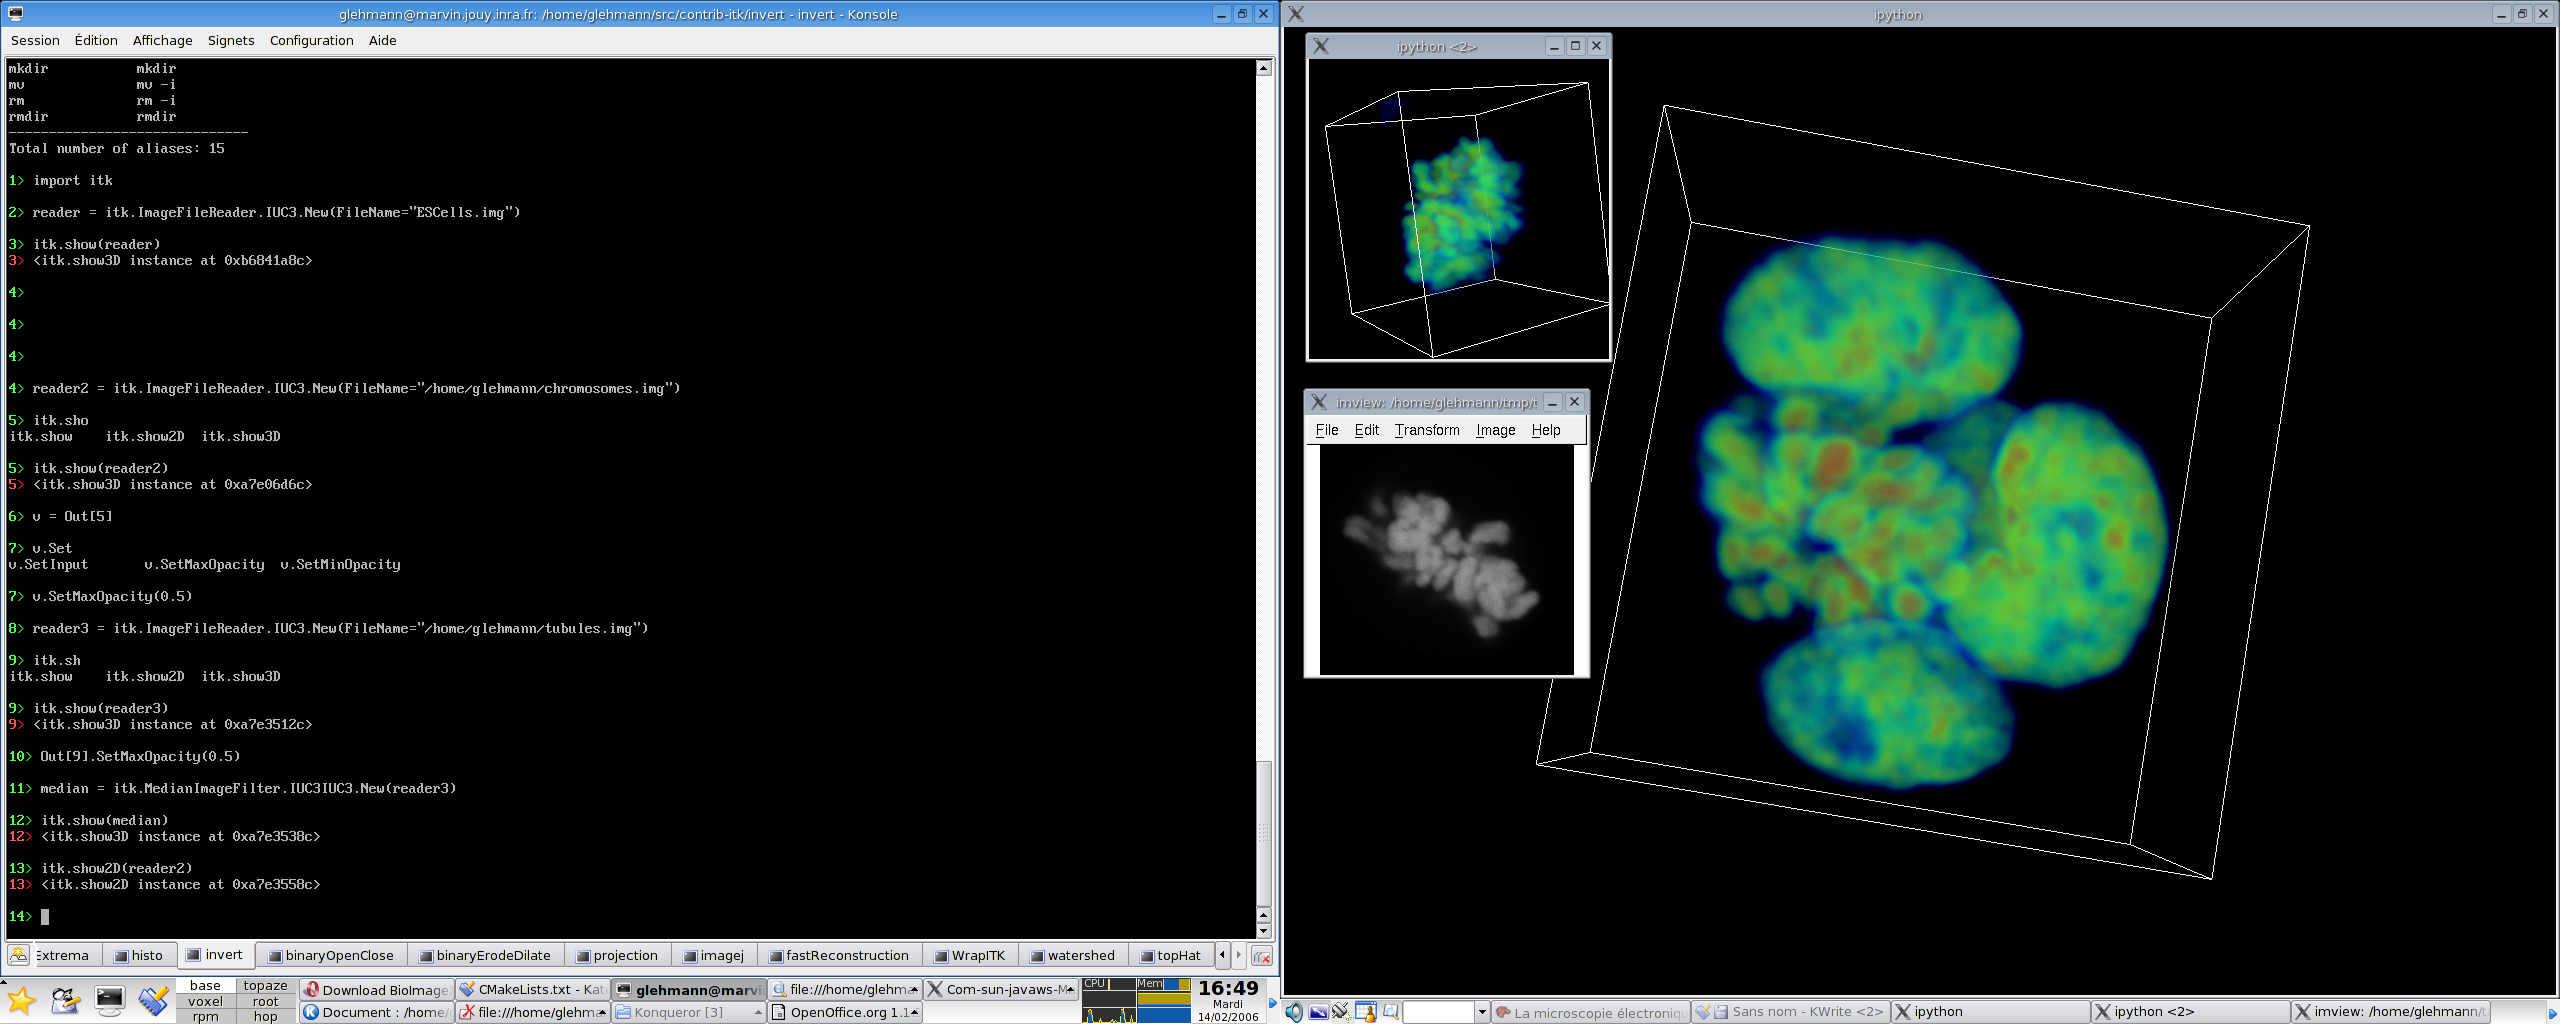
\includegraphics[scale=0.18]{capture1}
\caption{A screenshot of WrapITK in action with python.\label{screenshot}}
\end{figure}

  \item \verb$itk.strel(d, s)$ is used to create a binary ball structuring of dimension
\verb$d$ and size \verb$s$. Structuring element support is quite bad currently in WrapITK
and should change in the future. Using \verb$itk.strel$ rather than creating a
\verb$BinaryBallStructuringElement$ directly is recommended to have backward compatibility
when the structuring element type will be changed.

  \item \verb$itk.auto_progress(b)$ is used to automatically add a progress report
to all the newly created filters. \verb$b$ must be \verb$True$ or \verb$False$. If
\verb$b$ is true, something like
\begin{verbatim}
9> median.Update()
itkMedianImageFilterIF2IF2: 0.109990
\end{verbatim}
is displayed on the standard output. 
While prototyping, it is a convenient way for the user to know if
the execution time will be short or if he can do something more useful
\footnote{like having a cup of tea} than waiting for the filter to complete.

  \item \verb$itk.class_(object)$ return the class of an object. The \verb$__class__$
attribute is often not what the user want with ITK. \verb$itk.class_$ is a convenient
function to get the class of an ITK object.

Note that it is called \verb$class_$ and not \verb$class$, because \verb$class$ is a
reserved word in python.

Example:
\begin{verbatim}
10> median.__class__
10> <class 'itkMedianImageFilter.itkMedianImageFilterIF2IF2_PointerPtr'>

11> itk.class_(median)
11> <class 'itkMedianImageFilter.itkMedianImageFilterIF2IF2'>
\end{verbatim}


\end{itemize}

     \subsubsection{Advanced Features}

As an extra bonus, it is possible to view the doxygen documentation for each
class as the python docstring. This string is available as:
\small \begin{verbatim}
print itk.Image.__doc__
\end{verbatim} \normalsize
or even better (if you use iPython)
\small \begin{verbatim}
itk.Image?
\end{verbatim} \normalsize

Several steps are necessary to obtain this nirvana, however. First, when
configuring the build in ccmake, you must set \verb$DOXYGEN_MAN_PATH$ to some directory
where man pages for the ITK classes will be created. Then, after the build, you
must run \verb$make_doxygen_config.py$ from within the \verb$Python$ directory in the build
directory, to collect information about the wrapped classes and create a doxygen
configuration file to make these man pages. Finally, run doxygen with that
configuration file. After these three simple steps, class docstrings will
contain the man page information. Note that this is limited to systems which
support the python \verb$commands$ module, and which have \verb$groff$ in the path. This
basically means anything but windows \cite{WindowsWebSite} will work. (Cygwin should work too.)

In addition (as mentioned above), WrapITK by default ensures that no bare
pointers are ever returned to python: instead reference-counting \verb$SmartPointer$s
are used. However, there may be times when extracting a bare pointer or creating
a new \verb$SmartPointer$ is necessary. To get a bare pointer from a smart pointer, use
the \verb$GetPointer()$ method, as in ITK proper. To create a new smart pointer, the
\verb$SmartPointer$ template proxy class can be used just as above:
\small \begin{verbatim}
smartPtr = itk.SmartPointer[itk.Image[itk.US, 2]](image.GetPointer())
\end{verbatim} \normalsize
or just
\small \begin{verbatim}
smartPtr = itk.SmartPointer[image](image.GetPointer())
\end{verbatim} \normalsize

\verb$itk$ module can be very long to import. The \verb$itkConfig$ module define
a \verb$ImportCallback$ method which will be called when each sub module is
imported in the import process. \verb$ImportCallback$ can be customized to report the
progress status of the import process. It must be a function that can take
the name of the library being imported as a parameter. Here is an example of a very
basic callback function which display the name of the submodule being imported on
the standard error output.
\small \begin{verbatim}
import sys, itkConfig
def stderr_callback(name):
  print >> sys.stderr, name
itkConfig.ImportCallback = stderr_callback
import itk
\end{verbatim} \normalsize


    \subsection{TCL usage}

Write me.

    \subsection{Java usage}

Write me.

\section{Developer guide}

What follows is a brief description of how the WrapITK build system works, how
it can be extended, and how to write external projects.

  \subsection{WrapITK description}

     \subsubsection{Creating a CMakeLists.txt file for a wrapper library}
Each WrapITK sub-library (e.g. \verb$ITKCommonA$, or \verb$ITKAlgorithms$) lives in a
sub-directory of the WrapITK project (e.g. \verb$CommonA$ or \verb$Algorithms$) with a
\verb$CMakeLists.txt$ file that describes how that library  and language support files
(e.g. python template definitions) is to be created. Moreover, any external
project will need a similar file to describe how to create that library.

See \verb$SampleCMakeLists.txt$ in this directory for a description of each macro and
option that can appear in such a file. What follows is the usual set of commands
that will appear:

\small \begin{verbatim}
BEGIN_WRAPPER_LIBRARY("MySpatialObjectExtensions")
SET(WRAPPER_LIBRARY_DEPENDS ITKSpatialObject ITKCommonA)
SET(WRAPPER_LIBRARY_LINK_LIBRARIES ITKCommon)
WRAPPER_LIBRARY_CREATE_WRAP_FILES()
WRAPPER_LIBRARY_CREATE_LIBRARY()
\end{verbatim} \normalsize

\begin{itemize}
  \item \verb$BEGIN_WRAPPER_LIBRARY()$ sets up the environment to wrap a set of classes into a
library with a given name. This macro is defined in \verb$ConfigureWrapping.cmake$
\verb$WRAPPER_LIBRARY_DEPENDS$ stores the list of WrapITK libraries on which the
current library depends (e.g. which libraries wrap classes like \verb$Image$ or
\verb$SpatialObject$, that are going to be used in the current library). Every project
should at least depend on \verb$ITKCommonA$.

  \item \verb$WRAPPER_LIBRARY_LINK_LIBRARIES$ stores a set of other libraries to add at link
time. This can be 3rd party libraries that you will use (be sure to properly set
\verb$LINK_DIRECTORIES$ in this case), or more commonly, the ITK libraries that need to
be linked in, like \verb$ITKCommon$, \verb$ITKIO$, or other. 

  \item \verb$WRAPPER_LIBRARY_CREATE_WRAP_FILES()$ scans all of the \verb$wrap_XXX.cmake$ files in the
current directory and uses the directives within to create CableSwig input files
for these classes. Information about template instantiations is also recorded
for the language support files that are created next. This macro is defined in
\verb$CreateCableSwigInputs.cmake$, and calls language support macros from
\verb$CreateLanguageSupport.cmake$.

  \item Finally, \verb$WRAPPER_LIBRARY_CREATE_LIBRARY()$ creates rules to parse the CableSwig
inputs and compile a wrapper library. This macro also causes various language
support files to be created (python only currently) which make it easy to load
that library in python, and which know about the template instances defined.
This macro is defined in \verb$CreateWrapperLibrary.cmake$, and calls language support
macros from \verb$CreateLanguageSupport.cmake$.
\end{itemize}


     \subsubsection{Creating wrapXXX.cmake files to wrap classes}

A \verb$wrap_XXX.cmake$ file defines a group of classes and/or template instantiations
to be wrapped. Often one such file is defined for each class wrapped, but this
is not strictly necessary.

Within such a file, directives are issued to wrap classes and particular
template instances. 

WrapITK define several macros and variable designed to:
\begin{itemize}
  \item make creation of wrappers easy. The syntax is simple enough to get in quickly.
  \item make choice of template arguments explicit. It should be easy to understand
the idea of the author of a wrapper by reading the file.
  \item support mostly transparently the dimensions and types chosen by the user.
\end{itemize}

The most common case should be to create a new wrapper for a simple image filter, like 
\verb$MedianImageFilter$. Let see that example in details.

Here is the \verb$BasicFiltersB/wrap_itkMedianImageFilter.cmake$ file:

\small \begin{verbatim}
WRAP_CLASS("itk::MedianImageFilter" POINTER)
  WRAP_IMAGE_FILTER_INT(2)
  WRAP_IMAGE_FILTER_SIGN_INT(2)
  WRAP_IMAGE_FILTER_REAL(2)
END_WRAP_CLASS()
\end{verbatim} \normalsize

The file contains a \verb$WRAP_CLASS$ - \verb$END_WRAP_CLASS$ block, which itself contains
some \verb$WRAP_IMAGE_FILTER_*$ macros. \verb$WRAP_CLASS("itk::MedianImageFilter" POINTER)$
begin the wrapping of the \verb$itk::MedianImageFilter$ templated class. The name of the class
must be fully qualified. The option \verb$POINTER$ indicate that the object of the class can be
manipulated with a \verb$SmartPointer$, and that the \verb$SmartPointer$ specialization for
the class \verb$itk::MedianImageFilter$ must be created.

Then, several \verb$WRAP_IMAGE_FILTER_*$ macros are called. They are convenient macro to
create wrapper for classes which take only image types as template arguments. The parameter,
here \verb$2$, give the number of required template arguments. The two image types used as
template parameter are the same.

All of the available directives are defined and documented
in \verb$CreateCableSwigInputs.cmake$. The basics are presented here:

\begin{itemize}
  \item \verb$WRAP_CLASS("fully_qualified::ClassName" [POINTER|POINTER_WITH_SUPERCLASS])$
causes a templated class to be wrapped. All namespaces must be included in the
class name, and note that no template instantiation is given. Template
instantiations are created with various \verb$WRAP$ directives, described below,
between invocations of \verb$WRAP_CLASS()$ and \verb$END_WRAP_CLASS()$.

\verb$WRAP_CLASS("itk::ImageFilter")$ issues an implicit call to \verb$WRAP_INCLUDE("itkImageFilter.h")$, so the header
for the wrapped class itself does not need to be manually included. To disable
this behavior, set \verb$WRAPPER_AUTO_INCLUDE_HEADERS$ to \verb$OFF$.

The final optional parameter to \verb$WRAP_CLASS$ is \verb$POINTER$ or
\verb$POINTER_WITH_SUPERCLASS$. If no options are passed, then the class is wrapped
as-is. If \verb$POINTER$ is passed, then the class and the typedef'd \verb$class::Pointer$
type is wrapped. (\verb$Class::Pointer$ had better be a \verb$SmartPointer$ instantiation, or
things won't work. This is always the case for ITK-style code.) If
\verb$POINTER_WITH_SUPERCLASS$ is provided, then \verb$class::Pointer$, \verb$class::Superclass$ and
\verb$class::Superclass::Pointer$ are all wrapped. (Again, this only works for
ITK-style code where the class has a typedef'd \verb$Superclass$, and the superclass
has \verb$Self$ and \verb$Pointer$ typedefs). \verb$POINTER_WITH_SUPERCLASS$ is especially
useful for wrapping classes whose superclasses depend on the template definitions of the given
filter. E.g. any of the functor image filters, which define  totally different superclass
template parameters depending on which functor is used.

  \item \verb$END_WRAP_CLASS()$ -- end a block of template instantiations for a particular
class.

  \item \verb$WRAP_INCLUDE("header.h")$. By default, \verb$itkMedianImageFilter.h$ is included
when the  causes the \verb$itk::MedianImageFilter$ is wrapped, and this behavior is most of the
time enough. If it not enough, this macro can be used to include some specific files.

  \item \verb$WRAPPER_AUTO_INCLUDE_HEADERS$. This variable is set to \verb$ON$ by default, but can
be set to \verb$OFF$ to disable the auto include feature. This feature should be used when several
classes to wrap come from the same header file.
\verb$WRAPPER_AUTO_INCLUDE_HEADERS$ is re-set to \verb$ON$ for each new \verb$wrap_xxx.cmake$ file.

  \item \verb$WRAP_TEMPLATE("mangled_suffix" "template parameters")$. When issued between \verb$WRAP_CLASS$
and \verb$END_WRAP_CLASS$, this command causes a particular template instantiation of
the current class to be wrapped. The parameter \verb$mangled_suffix$ is a suffix to
append to the class's name that uniquely identifies this particular template
instantiation, and "template parameters" are whatever should go between the \verb$< >$
template instantiation brackets. (Do not include the brackets.) If you are
wrapping a filter, there are simpler macros to use, which are defined at the
bottom of \verb$CreateCableSwigInputs$ and described below.

  \item \verb$WRAP_NON_TEMPLATE_CLASS("fully_qualified::ClassName" [POINTER|POINTER_WITH_SUPERCLASS])$.
Same as \verb$WRAP_CLASS$, but creates a wrapper
for a non-templated class. No \verb$END_WRAP_CLASS()$ is necessary after this macro
because there is no block of template instantiating commands to close.

\end{itemize}

WrapITK define some lists which group the types and dimensions. Those list can be used
by the developer to create a wrappers but must {\em never} be modified.

\begin{itemize}
  \item \verb$WRAP_ITK_DIMS$ contains all the dimensions selected by the user.

  \item \verb$WRAP_ITK_INT$ contains all unsigned integer types selected by the user.

  \item \verb$WRAP_ITK_SIGN_INT$ contains all signed integer types selected by the user.

  \item \verb$WRAP_ITK_INTEGRAL$ contains all signed and unsigned integral types
selected by the user.

  \item \verb$WRAP_ITK_REAL$ contains all the real types selected by the user.

  \item \verb$WRAP_ITK_SCALAR$ contains all the scalar types selected by the user.

  \item \verb$WRAP_ITK_RGB$ contains all the \verb$RGB$ types selected by the user.

  \item \verb$WRAP_ITK_VECTOR_REAL$ contains all the \verb$Vector$ types selected
by the user.

  \item \verb$WRAP_ITK_COV_VECTOR_REAL$ contains all the \verb$CovariantVector$ types selected
by the user.

  \item \verb$WRAP_ITK_VECTOR$ contains all the \verb$Vector$ and 
\verb$CovariantVector$ types selected by the user.

  \item \verb$WRAP_ITK_ALL_TYPES$ contains all the types selected by the user.

  \item \verb$SMALLER_THAN_D$ contains all the types "smaller" than \verb$double$
selected by the user. This variable is useful when a filter decrease the range
of pixel value, like \verb$BinaryThresholdImageFilter$.

  \item \verb$SMALLER_THAN_UL$ contains all the types "smaller" than \verb$unsigned long$
selected by the user.

  \item \verb$SMALLER_THAN_US$ contains all the types "smaller" than \verb$unsigned short$
selected by the user.

  \item \verb$SMALLER_THAN_SL$ contains all the types "smaller" than \verb$signed long$
selected by the user.

  \item \verb$SMALLER_THAN_SS$ contains all the types "smaller" than \verb$signed short$
selected by the user.

\end{itemize}

WrapITK provides some macros to manipulate those list and use them
to create the wrappers. Most of those macros are there to fill a lack
of feature to manipulate lists in CMake, and should be replaced by
some CMake native commands in the future.

\begin{itemize}
  \item \verb$UNIQUE()$

  \item \verb$SORT()$

  \item \verb$INTERSECTION()$

  \item \verb$FILTER()$

  \item \verb$FILTER_DIMS()$

  \item \verb$INCREMENT()$

  \item \verb$DECREMENT()$

\end{itemize}


Some convenient macros are available to wrap image filters.

These macros often take an optional second parameter which is a "dimensionality
condition" to restrict the dimensions that the filter will be instantiated
for. The condition can either be a single number indicating the one dimension
allowed, a list of dimensions that are allowed (either as a single \verb$-$delimited
string or just a set of separate parameters), or something of the form \verb$n+$
(where \verb$n$ is a number) indicating that instantiations are allowed for dimension
n and above.


\begin{itemize}

  \item \verb$WRAP_IMAGE_FILTER_type(size)$ . \verb$type$ can be one of:
  \begin{itemize}
    \item \verb$INT$
    \item \verb$SIGN_INT$
    \item \verb$REAL$
    \item \verb$VECTOR_REAL$
    \item \verb$COV_VECTOR_REAL$
    \item \verb$RGB$
    \item \verb$ALL$
    \item \verb$SCALAR$
    \item \verb$VECTOR$
  \end{itemize}

 This macro create a template instantiation with \verb$size$
\verb$itk::Image$ parameters of the given pixel type. So if you are wrapping a filter
which should take two images with integral pixel types, write \verb$WRAP_IMAGE_FILTER_INT(2)$. The
specific integral data type(s) (\verb$char$, \verb$long$, or \verb$short$ in the \verb$WRAP_IMAGE_FILTER_INT$ case) will
be determined by the user-selected build parameters (e.g. \verb$WRAP_long$, and
\verb$WRAP_short$).

  \item \verb$WRAP_IMAGE_FILTER(param_types param_count)$ is a more general
macro for wrapping image filters that need one or more image parameters of the
same type. The first parameter to this macro is a list of image pixel types for
which filter instantiations should be created. The second is a \verb$param_count$
parameter which controls how many image template parameters are created. The
optional third parameter is a dimensionality condition.

E.g. \verb@WRAP_IMAGE_FILTER("${WRAP_ITK_ALL}" 2)@ will create template instantiations
of the filter for every pixel type that the user has selected.


  \item \verb$WRAP_IMAGE_FILTER_TYPES()$. Creates template instantiations of the
current image filter, for all the dimensions selected by the user (or dimensions
selected by the user that meet the optional dimensionality condition). This
macro takes a variable number of arguments, which should correspond to the image
pixel types of the images in the filter's template parameter list. The optional
dimensionality condition should be  placed in the last parameter.

  \item \verb$WRAP_IMAGE_FILTER_COMBINATIONS()$ takes a variable number of
parameters. Each parameter is a list of image pixel types. Filter instantiations
are created for every combination of different pixel types in different
parameters. A dimensionality condition may be optionally specified as the first
parameter. E.g. \verb$WRAP_IMAGE_FILTER_COMBINATIONS("UC;US" "UC;US")$ will
create: \verb$filter<itk::Image<unsigned char, d>, itk::Image<unsigned char, d> >$,
\verb$filter<itk::Image<unsigned char, d>, itk::Image<unsigned short, d> >$,
\verb$filter<itk::Image<unsigned short, d>, itk::Image<unsigned char, d> >$, and
\verb$filter<itk::Image<unsigned short, d>, itk::Image<unsigned short, d> >$
where \verb$d $is the image dimension, for each selected image dimension.

%   \item \verb$WRAP_type_DIMS(size dims)$ (with \verb$type$ as above) -- Wrap a filter for certain
% dimensions only. Dims should be either a semicolon-separated list of valid
% dimensions, or something of the form \verb$'3+'$ to specify that the filter can be
% instantiated only for three- and higher-dimensional images. Note that if the
% user has not selected to wrap a given dimension at build time, a filter wrapped
% with \verb$WRAP_type_DIMS$ will not be instantiated: the final dimensions wrapped are
% the {/em intersection} of the user-selected dimensions and the valid dimensions
% declared with \verb$WRAP_type_DIMS$.

\end{itemize}


  \subsection{Extending or customizing WrapITK}

To minimize build times and library size, it is possible to manually prevent
various classes from being wrapped. WrapITK is divided into several
sub-libraries, each with a sub-directory: \verb$Algorithms$, \verb$BasicFilters[ABC]$,
\verb$Common[AB]$, \verb$IO$, \verb$Numerics$, \verb$SpatialObject$, and \verb$VXLNumerics$. Within these
directories are sets or \verb$wrap_XXX.cmake$ files, where \verb$XXX$ is the name of the class
(or set of classes) to be wrapped. To prevent one of these classes from being
wrapped, simply rename the file to anything that does {\em not} start with \verb$wrap_$ and
end with cmake. (E.g. append \verb$.notwrapped$ to the name.) (This is probably
unsafe to do in the \verb$Common$, \verb$Numerics$, or \verb$IO$ directories.)

To add classes to be wrapped, it is recommended that you create a simple
{\em External Project} described below. If this is out of the question, you could
create additional \verb$wrap_XXX.cmake$ files in the appropriate directory. (Read on
for instructions as to what to put in these files.)


  \subsection{External projects}

    \subsubsection{Why external projects?}

External projects let the developer access some custom class with the target languages
and is a powerful way to extend WrapITK, test new wrapper, wrap more types, etc.
A nice side effect of wrappers, for contributions\footnote{A nice template for
contributions to the Insight Journal \cite{InsightJournalWebSite} which include the 
template code to build wrappers is available at
\url{http://voxel.jouy.inra.fr/darcs/contrib-itk/template/}. Just use the command
{\em darcs get http://voxel.jouy.inra.fr/darcs/contrib-itk/template/ contribName}
and edit the project name in the {\em CMakeLists.txt} file to
begin your new contribution.} for example, is to build {\em all}
the methods of the wrapped classes, and so to be sure everything builds as it should
\footnote{We have found and fixed numbers of bug in ITK while adding
more classes to WrapITK}.


    \subsubsection{Building}
To build an external project, first ensure that WrapITK has been properly built.
Then use \verb$ccmake$ to configure a build directory for the external project. If
WrapITK has not been installed, you will have to manually enter the path to the
WrapITK build directory.

By default, the build options are the same than the one used for building WrapITK,
but can be modified in the advanced options.

    \subsubsection{Usage}
Once an external project has been built, it can be tested directly from the
build tree. Start python in the external project build directory's Python
subdirectory, and run the command \verb$import ProjectConfig$ (or 
\verb$import ProjectConfig-[Debug|Release|...]$ if you were using an IDE, depending on which
build configuration was set from the IDE). This command sets up the search paths
properly so that WrapITK and the newly-created library files can be found. Then
type \verb$import ...$ (where \verb$...$ is replaced with the name of the external
project; e.g. \verb$import BufferConversion$), and use the project.

    \subsubsection{Installation}
Simply type \verb$make install$ (or run your IDE's install step) to install the
external project into the WrapITK tree (provided WrapITK has already been
installed). Now the external project can be used just like any of the other
WrapITK libraries, and it will be imported into the \verb$itk$ namespace when the
\verb$import itk$ command is issued from Python. (This can be disabled by setting
\verb$WRAPPER_LIBRARY_AUTO_LOAD$ to \verb$OFF$ in the external project's \verb$CMakeLists.txt$.)

    \subsubsection{Top-level CMakeLists for external projects}
In addition to having a set of \verb$wrap_XXX.cmake$ files and the proper
commands to read in these files and create a library (all described above), an
external project's CMakeLists file needs at least one additional command to
start it out: \verb$FIND_PACKAGE(WrapITK REQUIRED)$.

This command will cause cmake to try to find the WrapITK build/install
directory. If WrapITK has been installed, this will work on the first try.
Otherwise, you will have to set (within ccmake, or in the CMakeLists if you
prefer) the variable \verb$WrapITK_DIR$ to contain the path to the WrapITK build
directory.

    \subsubsection{Examples}

In \verb$WrapITK/ExternalProjects$ there are several sample "External Projects" that
can be built to provide additional functionality to WrapITK and to serve as a
demonstration for how to create your own such projects. One project is an
ITK-VTK \cite{VtkWebSite} bridge, and the other is a Python class to allow conversion from
Numeric/Numarray/numpy \cite{NumericWebSite,NumarrayWebSite,NumpyWebSite} matrices to
ITK images (and vice-versa).

More examples can be found in the contributions to the Insight Journal
\cite{InsightJournalWebSite}, or directly at \url{http://voxel.jouy.inra.fr/darcsweb/}.

    \subsubsection{BufferConversion: an example of extension for one language}

Write me.

    \subsubsection{ItkVtkGlue: an example of extension for all languages, including C++}

ItkVtkGlue wrap the classes used to convert data from ITK to VTK \cite{VtkWebSite} and from VTK to ITK.
Those classes comes from the InsightApplications \cite{ITKWebSite}, and make the conversion
as simple in python as in C++. It has been tested with VTK 5.0.0.

By default, those classes are not loaded in the \verb$itk$ module to avoid loading
all the \verb$vtk$ module while importing \verb$itk$. The command \verb$import itkvtk$
will load the module, and add the classes both in \verb$itkvtk$ and \verb$itk$ module.
The classes are then usable as the other itk classes.

Example:
\begin{verbatim}
1> import itk

2> import itkvtk

3> reader = itk.ImageFileReader.IUC3.New()

4> converter = itk.ImageToVTKImageFilter.IUC3.New(reader)

5> converter.GetOutput()
5> <libvtkFilteringPython.vtkImageData vtkobject at 0xb7675b60>
\end{verbatim}


The \verb$itk.show3D$ class use the class \verb$ImageToVTKImageFilter$ to create the
volume rendering shown in Figure \ref{screenshot}.

  \subsection{Extending language support and adding more languages}

Write me.

    \subsubsection{Generating target language code}

Write me.

    \subsubsection{typemaps}

Write me.

  \subsection{Contributing to WrapITK}

WrapITK is an opensource project, and so all contributions are welcome. Here are
some points which requires special attention:
\begin{itemize}
  \item Test it and report problem. That's the more important thing to do:
we need feedbacks to enhance WrapITK quality ! Report all bugs you may found
to \url{http://voxel.jouy.inra.fr/roundup/wrapitk/} \cite{RoundupWebSite}.
  \item Work on tcl, java, and others. We are not tcl or java developers, and so
are not able to complete the work for those languages. Any help from tcl and
java expert would be highly appreciated. Also, there is no reason to be limited
to python, tcl and java, and WrapITK can be extended to other languages supported
by swig like perl \cite{PerlWebSite}, ruby \cite{RubyWebSite}, ocaml \cite{OcamlWebSite} and others.
  \item Add more classes. WrapITK add lots of new classes compared to the current
wrapping system, but there is still lots of work to do, especially to support more
filter dedicated to \verb$Vector$ pixels.
\end{itemize}

\verb$darcs$ \cite{DarcsWebSite} allow to easily contribute to WrapITK, by sending patch by email with
the command \verb$darcs send$, while keeping credits for the work done.
Feel free to send patches; they will be tested and integrated in the project.

A web interface \cite{DarcswebWebSite} for the WrapITK's darcs
repository is available at \url{http://voxel.jouy.inra.fr/darcsweb/}.


\section{Acknowledgments}
I thank Dr Pierre Adenot and all the {\em Embryon et Biotechnologie} team for their
patience during the long development time before getting a tool really usable.

We would like to thank Charl P. Botha for is help to debug WrapITK on windows
plateform, and for the patches he has contributed, as well as Richard Beare for
his early interest in using itk with python, for his useful feedbacks, and for
his work on buffer conversion in python.

We thank Brad King for his assistance during the development process.

Finally, we thank the ITK developers for the great tool which is ITK, and for the
previous work done on wrapping system - without it WrapITK would not be there.


\section{Conclusion}

ITK is a great library, with the drawback to be nearly unusable for prototyping,
and to have a poor support for other languages than C++. WrapITK address those
issue and finally give to ITK a quite good support for python. We hope that support
will soon be extended to tcl and java.



\appendix



\bibliographystyle{plain}
\bibliography{Article,InsightJournal}
\nocite{ITKSoftwareGuide}

\end{document}

